\chapter{Harmonic Onset Detector Algorithm}

An ideal onset detection algorithm would detect all the played notes and eliminate all noises. The algorithm can be built on the differences between the noises and musical notes.   

All events, noises and notes, introduce changes to the energy distribution of the frequencies. Some events, may not cause an increase of the total energy. For example, during a glissando, the played note changes without an energy increase. Therefore, frequency domain representation of the audio signal is suitable for detecting guitar (and many other pitched instruments) note onsets. Crucial step is to find the differences of noises and notes in that representation.

Most useful property of guitar notes is that they are harmonic. This property can be exploited to separate notes from various inharmonic noises. For slide and buzz noises, which are harmonic, further inspection is needed. Unstability of the frequencies of the slide noises can be used to eliminate slide noises. Fundamental frequency (f0) of the sound event can also be used for determining a note, fundamental frequency of a slide noise is usually greater than f0 of possible guitar notes. For example, average of the hand speed in the slide noise shown in Figure \ref{fig:slide} is approximately 0.45 m/s (distance between frets divided by slide duration) and average fundamental frequency is 1800 Hz (using the equation \ref{slide_eq}, \(d_w \approx 4000 \) windings per meter). A slide noise with faster hand speed can surpass the highest possible fundamental frequency on a guitar with standard tuning, which is 1975 Hz (B6). In the case of buzz noises, frequencies of the harmonics are stable. Most distinguishable property of buzz noises is their duration are quite short compared to notes. Figure \ref{fig:buzz} shows a buzz noise that lasts around 0.1 seconds. That buzz is generated intentionally and is quite longer than buzz noises found in performance. In Figure \ref{fig:realbuzz} we see a naturally occurring buzz noise in a beginners performance. Given the properties of notes and noises, an onset detection algorithm can be built according to following argument: \\ At a given time point, a guitar note onset exists if there is at least one harmonic series in the differences of energy magnitudes of frequencies after and before the time point, and that harmonic series lasts longer than minimum expected note duration. There are more than one ways to create an algorithm to detect guitar notes in the way they are described in the argument above. In the remaining of this section, design and parameter choices of the developed algorithm is discussed.

Detecting and tracking the harmonic series requires a time-frequency representation of the audio signals. Short-time Fourier Transform is the first step of the algorithm. Detecting harmonic series on a time frame requires calculations over peaks of the spectrum, which will be called the \textit{harmonic analysis} step. Duration of a harmonic series is calculated by tracking the harmonic series through successive time frames, which is called the \textit{segmentation} step. Those two steps (harmonic analysis and segmentation) brings computational expense. Applying them on every time frame is not practically possible. Therefore an \textit{onset candidate selection} step is required before those steps. The candidate selection step should be much cheaper, as it is applied to all time frames. Details of each step is described in following sections. The overall algorithm consisting those steps is referred as Harmonic Onset Detector.

\begin{figure}
    \centering
    
\includegraphics[width=\columnwidth]{methods/overall.png}
    \caption{Overall scheme of Harmonic Onset Detector algorithm.}
    \label{fig:scheme}
\end{figure}

\section{Short-Time Fourier Transform}
Separating lower frequencies require a larger window size, but a large window size causes smoothing in time, decreasing the time accuracy of the onset detection algorithm. Using different window sizes for different frequency bands solves this problem at the expense of computation. The following parameters are found to be working well in experiments.

Bands (Hz): (0-1000), (1000-5000), (5000 - \(F_s / 2\)) \\
Window Sizes: 8191, 2047, 1023\\
Window: Blackman
FFT Size = 8192\\
Hop Size = 128 

Where  \(F_s\) is the sampling rate. The window size of the lowest band is not large enough to separate the two closest frequencies on a guitar with standard tuning (82.41 Hz and 87.31 Hz). This does not prevent the detection of low frequency notes because the detection of the harmonic series is done with an error tolerance. Even if the fundamental frequency (f0) is not separated, higher harmonics (f1,f2...) are separated and the existence of a new harmonic series can be detected from those higher harmonics.

\section{Candidate Selection}

This step is required to avoid applying the rest of the algorithm on all time frames. Spectral flux \cite{spectralflux} is the sum of the positive differences of frequency magnitudes. It measures the positive change between consecutive time frames. Originally, the summation includes all frequency bins. Experiments showed that limiting the frequency bins between possible fundamental frequencies of guitar improves the performance of candidate selection. Bins are limited between two bins below the minimum frequency (82 Hz) and two bins above the maximum frequency (1975 Hz). Bins corresponding to these frequencies can be calculated using FFT size.

\begin{equation}\label{SF}
    SF(t) = \sum_{k=N_{82Hz}-2}^{N_{1975Hz}+2} H(|X(t,k)|-|X(t-1,k)|)
\end{equation}

Where $H$ is the half wave rectifier and $t$ denotes the time frame. SF is normalized between 0 and 1, \( SF = SF / \max |SF|\)  and then smoothed by using a Savitzky-Golay filter \cite{savgol} with window size (\(w_{SG}\)) of 51 and polynomial order of 3. The size of the window can be converted to time by multiplying with (Hop Size \(/ f_s\)), which is 0.148 ms in this case. The main contribution of this smoothing step is to reduce the number of candidates in strummed chords.

A simple peak picking algorithm is used on smoothed SF to select candidates. A time frame is selected as an onset candidate if SF(t) is maximum between the time window \((t-\lfloor w_{SG}/2\rfloor, t+\lfloor w_{SG}/2\rfloor) \) and is greater than the average inside that window by a small threshold of 0.01.  

\section{Harmonic Analysis}

STFT magnitudes after and before the onset candidate are compared to determine the existence of new harmonic series. 160 frames around onset candidates (80 left, 80 right) are used for the analysis. The analysis window shortens if there is another onset candidate closer than 80 frames (if not, an inharmonic noise just before a true onset would be falsely predicted as an onset).  Keeping the number of frames for analysis on the right side of the onset candidate is important for the accuracy of the algorithm. Onset candidates are therefore analysed starting from the latest and removed from the candidate list if they are not predicted as onsets, allowing the previous (in time) onset candidate to be analysed on 80 frames on the right side.

Two windows of frames just before and after the candidate are used to determine the frequencies that gained energy. The lengths of those windows are equal to half of the total number of analysis frames on each side. Windows are moved away from the onset candidate so they contain less smeared energy and frequencies with increased magnitude can be more accurately detected. The average magnitude of each frequency bin is calculated inside two windows and compared. Frequency bins that have not gained energy above a threshold are masked. So the algorithm only seeks for harmonic series inside the frequencies that gained energy. This way, an inharmonic noise will not be falsely predicted as an onset when there is already some harmonic content.

For each time frame, peaks on the spectrum are detected and another frequency masking is applied. Peaks are eliminated if they are close to a peak with much higher energy. The aim is to eliminate the perceptually masked frequencies and to reduce the computation of the harmonic series search. This perceptually motivated masking is not a realistic simulation of human perception, it is meant to be quite simple and computationally cheap. Figure \ref{fig:crude_mask} shows an example of the masking. 

From the remaining peak locations, the first 10 peaks in the range of the guitar are selected as f0 candidates. Possible missing f0 candidates are generated by dividing higher peak frequencies by 2 and 3, then added to the f0 candidate pool. Error for each harmonic series is calculated as follows:\\
$H$: Highest harmonic considered in the error calculation \\
\(D(nf0)\): distance of $n^{th}$ harmonic to the closest frequency peak \\
\(r(nf0)\): error of the $n^{th}$ harmonic \\
\(R(F0)\): total weighted error of the harmonic series

\begin{equation}\label{nerror}
    r(nf0)= \begin{cases} 
          D(nf0) & D(nf0)\leq 2n \\
          30 & D(nf0) > 2n 
          \end{cases}
\end{equation}  

If $D(nf0)$ is greater than $2n$, $n^{th}$ harmonic is marked as non-existent. After the error calculation of all harmonics (from 1 to H), error values are weighted using the equation (\ref{wnerror}), where $p$ is the number of harmonics that are found to be existent and $c$ is strictness constant. The total error of the harmonic series is the summation of weighted errors (\ref{toterror}). \

\begin{equation}\label{wnerror}
    r(nf0) =  r(nf0)\cdot e^{-n / e^{H-p+c}}
\end{equation}  
\begin{equation}\label{toterror}
    R(F0) =  \sum_{n=1}^{H} r(nf0)
\end{equation}

\begin{figure}
    \centering
    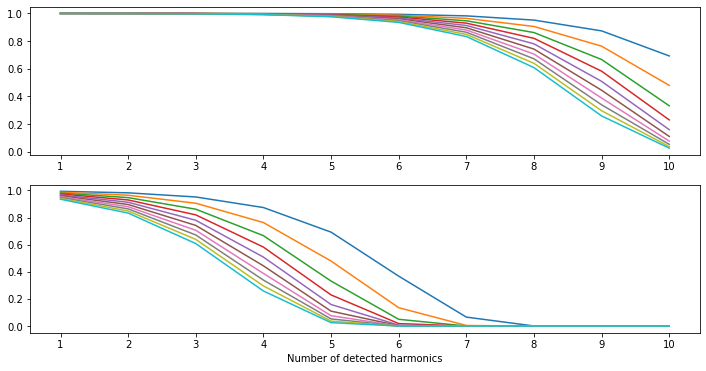
\includegraphics[width=\columnwidth]{methods/hweights.png}
    \caption{Weights of harmonic errors (top to bottom, $0^{th}$ to $(H-1)^{th}$ harmonic) w.r.t. number of existent harmonics. $H = 10$, $c = 0$ (above) and $c = -5$ (below). }
    \label{fig:hweights}
\end{figure}

Equation (\ref{fig:hweights}) adds two things to algorithm. First, the existence of a frequency peak close to a harmonic value is acknowledged directly, the total error decreases with the number of detected harmonics. Second, lower harmonics have more importance. The strictness constant ($c$) is chosen to be -1 in this algorithm. Figure \ref{fig:hweights} shows how $c$ affects the weights.

\section{Segmentation}

Detected harmonic series are tracked through successive frames. The existence of the harmonic series is decided by an error threshold, $t_{he}$. If a harmonic series exists in $n$ consecutive frames, it forms a segment of length $n$. In a segment, harmonic series are allowed to deviate from previous ones to neighboring series, making the segmentation robust against small frequency deviations. The total duration of a harmonic series is calculated by summing the length of its segments. Error and length thresholds are defined and explained below.

Harmonic series error threshold ($t_{he}$) = 200 \\
If the error of a harmonic series in a frame is below  $t_{he}$, it starts or continues the segment at the current frame. If it is above and there is a segment up to this frame, the segment ends. 

Segment error threshold ($t_{se}$) = 80 \\
If the average error of a harmonic series along a segment is greater than $t_{se}$, the segment is eliminated. $t_{he}$ is greater than $t_{se}$, which means higher errors are tolerated for single frames so the segments are not disrupted, but average error along the segments must be lower. 

A numerical example: if 3 harmonics of a series are missing for every frame on a segment and the remaining 7 harmonics are found without any distance error, the total unweighted error would be 90, surpassing the threshold. If the missing harmonics are $7^{th}$,$8^{th}$ and $9^{th}$, which have lower weights than the lower harmonics, total weighted error would be 76.3. In that case, the segment is not eliminated and its length is added to the total length.    \\\\
Segment length threshold ($t_l$) = 8 frames \\
If the length of a segment is less than $t_l$, the segment is eliminated. \\\\
Total length threshold ($t_L$) = 30 frames\\
If the total length of segments of a harmonic series is less than $t_L$, the harmonic series is not accepted as evidence of a guitar note. If it is greater or equal, the onset candidate is predicted as a note onset. 

If there is at least one harmonic series that satisfy the condition above (total length of the segments $\geq t_L$), the onset candidate is predicted as a guitar onset.

A guitar note and a buzz noise are shown in Figures \ref{fig:gs_0_note} and \ref{fig:gs_0_noise}. Both candidates are predicted correctly.

\begin{figure}
    \centering
    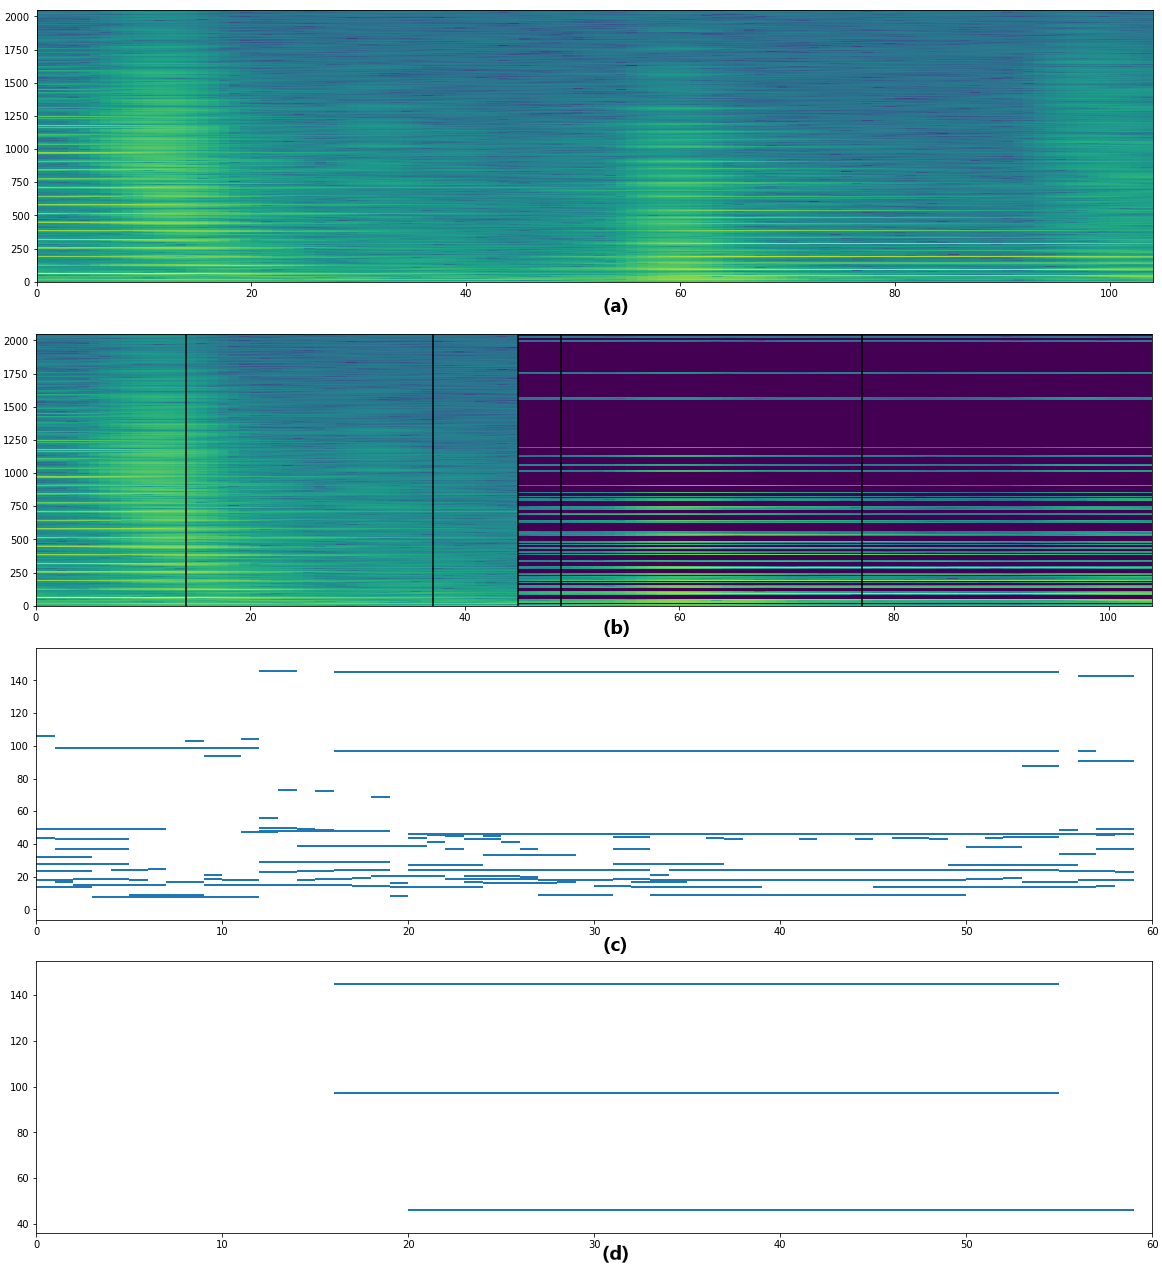
\includegraphics[width=\columnwidth]{methods/gs_0_788_note.png}
    \caption{Visualization of an onset candidate being processed (x: time frames, y: frequency bins). (a) STFT around the onset candidate, (b) Elimination of frequencies after the candidate. Middle line: onset candidate, two lines on both sides: boundaries for frequency elimination calculation. (c) Segments of harmonic series before error and duration thresholds are applied (the candidate is at time frame 0), (d) Remaining segments that are accepted as evidences of a note onset }
    \label{fig:gs_0_note}
\end{figure}

\begin{figure}
    \centering
    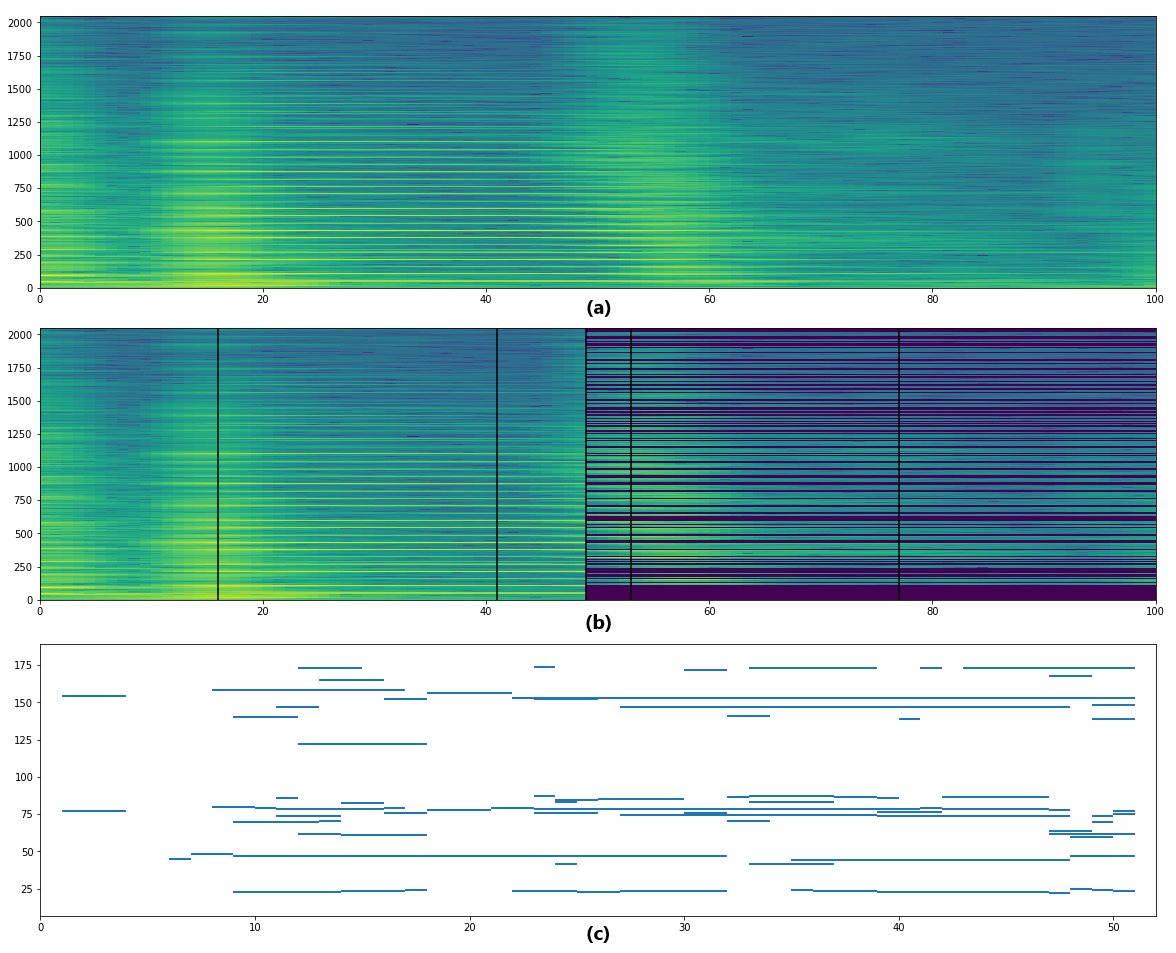
\includegraphics[width=\columnwidth]{methods/gs_0_642_noise.png}
    \caption{Visualization of an onset candidate being processed (x: time frames, y: frequency bins). (a) STFT around the onset candidate, (b) Elimination of frequencies after the candidate. Middle line: onset candidate, two lines on both sides: boundaries for frequency elimination calculation. (c) Segments of harmonic series before error and duration thresholds are applied (the candidate is at time frame 0). All segments are eliminated after thresholds are applied.}
    \label{fig:gs_0_noise}
\end{figure}

\begin{figure}
    \centering
    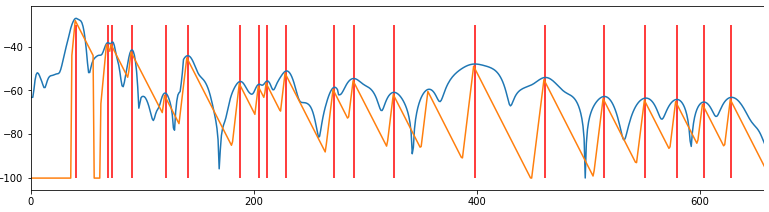
\includegraphics[width=\columnwidth]{methods/crude_masking_r.png}
    \caption{Elimination of frequency peaks in a single time frame. A triangle mask (orange) is created around each peak (red). Peaks that remain under mask are eliminated, such as the peak at 100 Hz.}
    \label{fig:crude_mask}
\end{figure}
